\section{Motivation}
    \begin{frame}{Linear regression model}
    Consider the usual linear regression model: given $p$ predictors $x_1,..., x_p$, the response $y$ is predicted by
    
    \begin{equation}
\hat{y} = \hat{\beta}_0 + x_1\hat{\beta}_1 + \ldots + x_p\hat{\beta}_p
\end{equation}
\vspace{10pt}
A model fitting procedure produces the vector of coefficients $\hat{\boldsymbol{\beta}}=\left(\hat{\beta}_0,...,\hat{\beta}_p\right)$. For example, the ordinary least squares (OLS) estimates are obtained by minimizing the residual sum of squares.
    \end{frame}

    \begin{frame}{Criteria}
        \begin{itemize}
            \item \textbf{Accuracy of prediction on future data}—it is difficult to defend a model that predicts poorly.
            \item \textbf{Interpretation of the model}—scientists prefer a simpler model because it puts more light on the relationship between the response and covariates.
        \end{itemize}
        \vspace{10pt}
        It is well known that OLS often does poorly in both prediction and interpretation.
\end{frame}

\begin{frame}{Penalization techniques to improve OLS}
    
    \begin{figure}
        \centering
        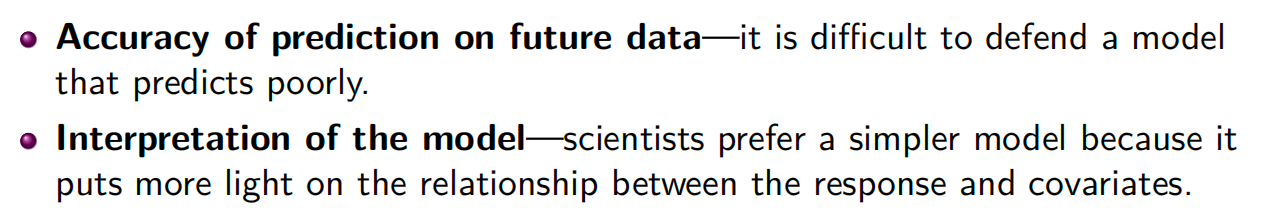
\includegraphics[width=1\textwidth]{img/image4.png}
    \end{figure}
    
    \begin{block}{Ridge regression}
     As a continuous shrinkage method, ridge regression achieves its better prediction performance through a bias–variance trade-off. However, ridge regression cannot produce a parsimonious model, for it always keeps all the predictors in the model.
    \end{block}
    
     \begin{block}{Best subset slection}
         Best subset selection in contrast produces a sparse model, but it is extremely variable because of its inherent discreteness.
     \end{block}
    \end{frame}

    \begin{frame}{Penalization techniques to improve OLS}
    \begin{block}{Lasso}
        The lasso does both continuous shrinkage and automatic variable selection simultaneously.
        \begin{itemize}
            \item In the $p>n$ case, the lasso selects at most $n$ variables before it saturates, because of the nature of the convex optimization problem.
            \item If there is a group of variables among which the pairwise correlations are very high, then the lasso tends to select only one variable from the group and does not care which one is selected.
            \item For usual n>p situations, if there are high correlations between predictors, it has been empirically observed that the prediction performance of the lasso is dominated by ridge regression.
        \end{itemize}
    \end{block} 
    \end{frame}

\section{Naive elastic net}
    \begin{frame}{Definition}
    Suppose that the data set has $n$ observations with $p$ predictors. Assume:
    \begin{equation}
        \sum_{i=1}^{n} y_i = 0, \quad \sum_{i=1}^{n} x_{ij} = 0 \quad \text{and} \quad \sum_{i=1}^{n} x_{ij}^2 = 1, \quad \text{for } j = 1,2,\ldots,p.
    \end{equation}
     For any fixed non-negative $\lambda_1$ and $\lambda_2$, we define the naive elastic net criterion
     \begin{equation}
         L(\lambda_1, \lambda_2, \boldsymbol{\beta}) = ||y - X\boldsymbol{\beta}||^2 + \lambda_2 ||\boldsymbol{\beta}||^2 + \lambda_1 ||\boldsymbol{\beta}||_1,
     \end{equation}
     where
     \[
||\boldsymbol{\beta}||^2 = \sum_{j=1}^{p} \beta_j^2,
\]
\[
||\boldsymbol{\beta}||_1 = \sum_{j=1}^{p} |\beta_j|.
\]
    \end{frame}

\begin{frame}{Definition}

The naive elastic net estimator $\hat{\beta}$ is the minimizer of equation (3):
\begin{equation}
\hat{\mathbf{\beta}} = \arg\min_{\mathbf{\beta}} L(\lambda_1, \lambda_2, \mathbf{\beta}).
\end{equation}
This procedure can be viewed as a penalized least squares method. Let $\alpha = \lambda_2 / (\lambda_1 + \lambda_2)$, then solving $\hat{\beta}$ in equation (3) is equivalent to the optimization problem

\vspace{10pt}

\begin{equation}
\begin{aligned}
\hat{\mathbf{\beta}} &= \underset{\mathbf{\beta}}{\arg\min} \ \|y - X\mathbf{\beta}\|^2, \\
&\text{subject to } (1 - \alpha) \|\mathbf{\beta}\|_1 + \alpha \|\mathbf{\beta}\|^2 \leq t \text{ for some } t.
\end{aligned}
\end{equation}

\end{frame}


    \begin{frame}{Definition}
        \begin{figure}
            \centering
            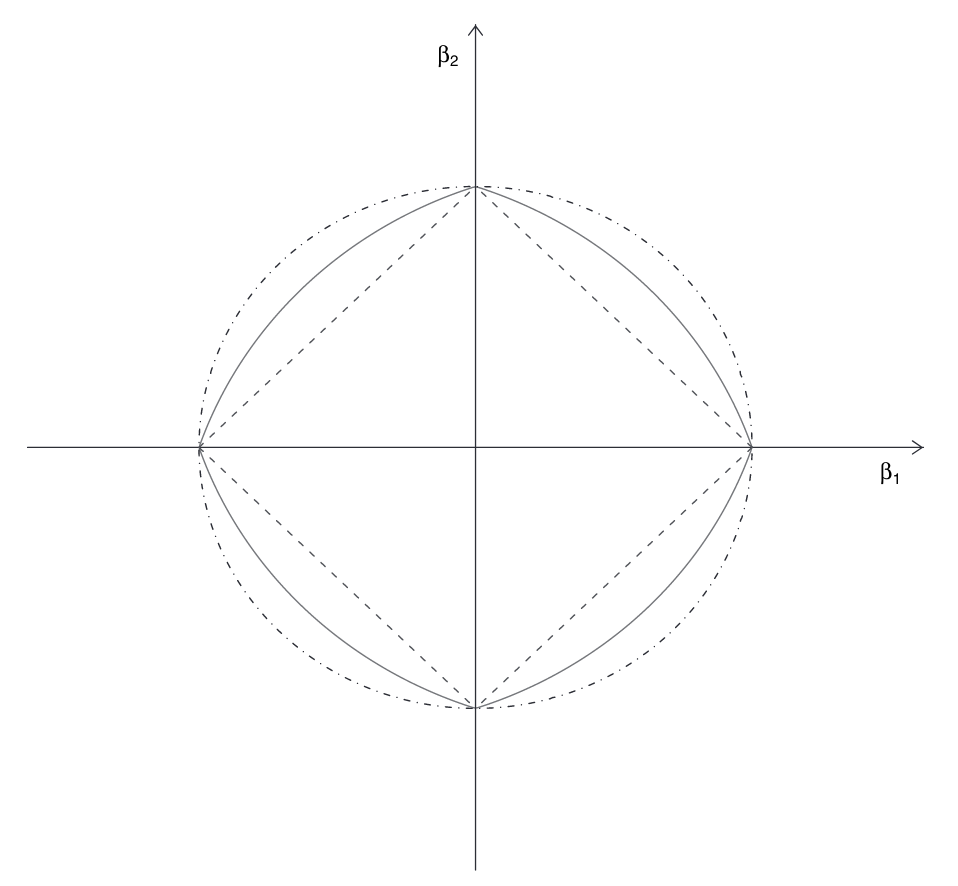
\includegraphics[width=0.6\textwidth]{img/image1.png}
            \caption{Two-dimensional contour plots}
        \end{figure}
    \end{frame}

    \begin{frame}{Solution}
        \begin{block}{LEMMA 1}
            Given data set $\left(\textbf{y}, \textbf{X}\right)$ and $(\lambda_1, \lambda_2)$, define an artificial data set $\left(\textbf{y}^*, \textbf{X}^*\right)$ by
$$
\mathbf{X}^*_{(n+p) \times p} = (1 + \lambda_2)^{-1/2}
\begin{pmatrix}
\mathbf{X} \\
\sqrt{\lambda_2} \mathbf{I}
\end{pmatrix}, \quad
\mathbf{y}^*_{(n+p)} = \begin{pmatrix}
\mathbf{y} \\
\mathbf{0}
\end{pmatrix}.
$$
Let $\gamma=\lambda_1/\sqrt{(1+\lambda_2)}$ and $\beta^*=\sqrt{(1+\lambda_2)}\beta$. Then the naive elastic net criterion can be written as
$$
L(\gamma, \beta) = L(\gamma, \beta^*) = \lVert y^* - X^* \beta^* \rVert_2^2 + \gamma \lVert \beta^* \rVert_1.
$$
Let
$$
\hat{\beta}^* = \underset{\beta^*}{\arg\min} L\left(\gamma, \beta^*\right); \quad \text{then} \quad \hat{\beta} = \frac{1}{\sqrt{(1 + \lambda_2)}} \hat{\beta}^*.
$$
\end{block}
\end{frame}

\begin{frame}{Solution - Orthogonal case}
    In the case of an orthogonal design, it is straightforward to show that with parameters $(\lambda_1, \lambda_2)$ the naive elastic net solution is

\begin{equation}
  \hat{\beta}_i (\text{naive elastic net}) = \frac{(|\hat{\beta}_i^{(OLS)}| - \lambda_1 / 2)_+}{1 + \lambda_2} \text{sgn}(\hat{\beta}_i^{(OLS)}) 
\end{equation}


where $\hat{\beta}^{(OLS)} = X^T y$ and $z_+$ denotes the positive part, which is $z$ if $z \geq 0$ and $0$ otherwise. The solution of ridge regression with parameter $\lambda_2$ is given by $\hat{\beta}^{(ridge)} = \hat{\beta}^{(OLS)} / (1 + \lambda_2)$, and the lasso solution with parameter $\lambda_1$ is

$$
\hat{\beta}_i (\text{lasso}) = |(\hat{\beta}_i^{(OLS)}| - \lambda_1 / 2)_+ \text{sgn}(\hat{\beta}_i^{(OLS)}).
$$

\end{frame}

\begin{frame}{Solution - Orthogonal case}
    \textbf{Proof:} In orthogonal case, $X^TX = 1$, so $\hat{\beta}^{OLS}=X^Ty$.
Given these conditions, the loss function \(L(\beta_i)\) is given by:

$$
L(\beta_i) = (y - \beta_i)^2 + \lambda_2 \beta_i^2 + \lambda_1 |\beta_i|,
$$

where \(y\) and \(\beta_i\) are elements of \(y\) and \(\beta\), respectively. If we represent \(z\) as $\beta_i$, then the loss function \(L(z)\) can be expanded as:

$$
L(z) = (z - \hat{\beta}_i^{(OLS)})^2 + \lambda_2 z^2 + \lambda_1 |z|,
$$

When $z \geq 0$,

$$
\frac{dL(z)}{dz} = 2(z - \hat{\beta}_i^{(OLS)}) + 2\lambda_2 z + \lambda_1 = 0
$$

\end{frame}

\begin{frame}{Solution - Orthogonal case}
    \textbf{(Continued)}  Given the above conditions, we deduce: $$ 
z^* = \frac{\hat{\beta}_i^{(OLS)} - \lambda_1 / 2}{1 + \lambda_2}
$$
When $z \leq 0$,
$$
L(z) = (z - \hat{\beta}_i^{(OLS)})^2 + \lambda_2 z^2 - \lambda_1 z
$$
Subsequently, to find the minimum of the loss function, we take the derivative with respect to \( z \) and set it to zero:

$$
\frac{dL(z)}{dz} = 2(z - \hat{\beta}_i^{(OLS)}) + 2 \lambda_2 z - \lambda_1 = 0
$$
\end{frame}

\begin{frame}{Solution - Orthogonal case}
    \textbf{(Continued)} Subsequently, to find the minimum of the loss function, we take the derivative with respect to \( z \) and set it to zero:

$$
\frac{dL(z)}{dz} = 2(z - \hat{\beta}_i^{(OLS)}) + 2 \lambda_2 z - \lambda_1 = 0
$$
The solution is:
$$
z^* = \frac{\hat{\beta}_i^{(OLS)} + \lambda_1 / 2}{1 + \lambda_2}
$$

\end{frame}

\begin{frame}{Solution - Orthogonal case}
    \begin{figure}
        \centering
        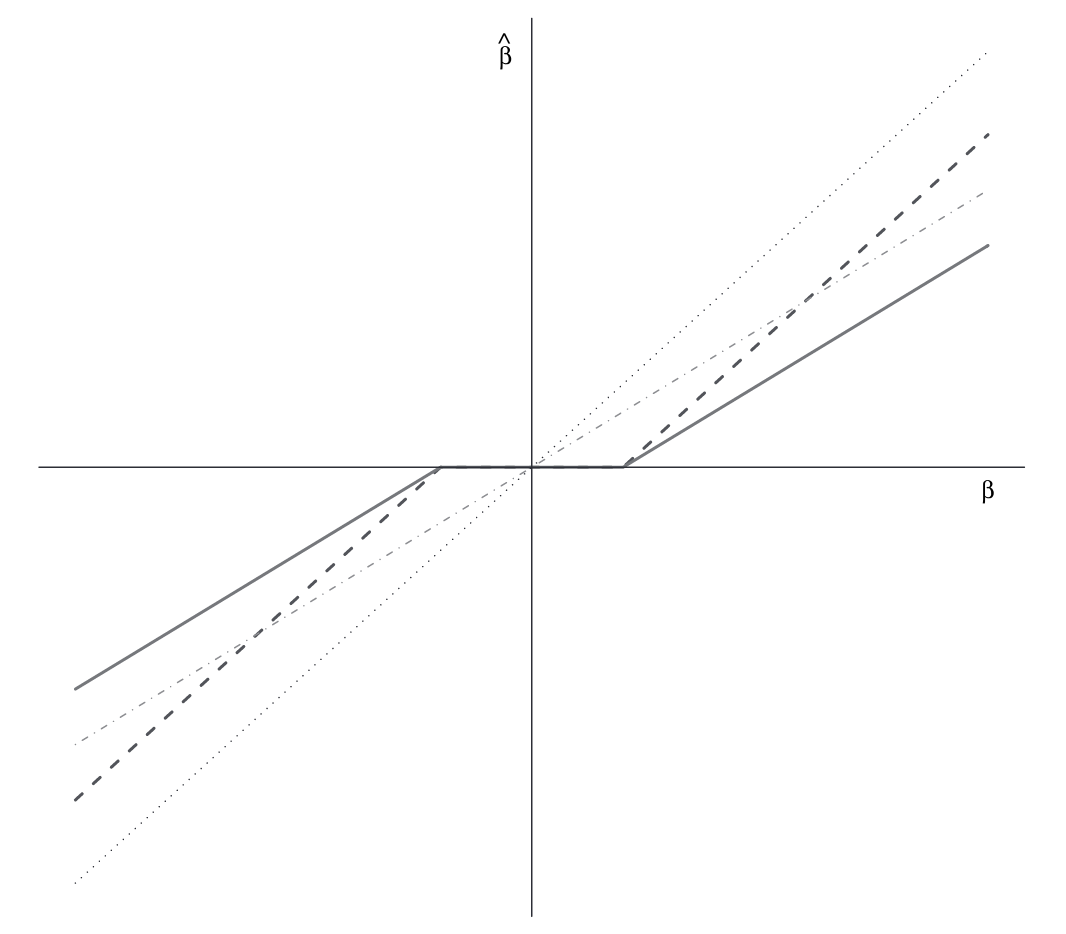
\includegraphics[width=0.6\textwidth]{img/image2.png}
        \caption{Exact solutions for the lasso, ridge regression and the naive elastic net in an orthogonal design}
    \end{figure}
\end{frame}

\begin{frame}{Grouping effect}
    We consider the generic penalization method
\begin{equation}
    \hat{\beta} = \underset{\beta}{\arg\min} \left\lVert y - X\beta \right\rVert^2 + \lambda J(\beta)
\end{equation}
    where $J(\cdot)$ is positive valued for $\beta \neq 0$.

\begin{block}{LEMMA 2}
        Assume that $\textbf{x}_i = \textbf{x}_j, i,j \in \{1, \ldots, p\}$.

1. If \( J(\cdot) \) is strictly convex, then \( \hat{\beta}_i = \hat{\beta}_j, \forall \lambda > 0. \)

2.  If \( J(\beta) = \lVert \beta \rVert_1 \), then \( \hat{\beta}_i \hat{\beta}_j \geq 0 \) and \( \hat{\beta}^* \) is another minimizer of equation (7), where

% \begin{enumerate}%[label=(\alph*)]
%   \item If \( J(\cdot) \) is strictly convex, then \( \hat{\beta}_i = \hat{\beta}_j, \forall \lambda > 0. \)
%   \item If \( J(\beta) = \lVert \beta \rVert_1 \), then \( \hat{\beta}_i \hat{\beta}_j \geq 0 \) and \( \hat{\beta}^* \) is another minimizer of equation (7), where
% \end{enumerate}

\[
\hat{\beta}_k^* = 
\begin{cases} 
\hat{\beta}_k & \text{if } k \neq i \text{ and } k \neq j, \\
(\hat{\beta}_i + \hat{\beta}_j) \cdot (s) & \text{if } k = i, \\
(\hat{\beta}_i + \hat{\beta}_j) \cdot (1 - s) & \text{if } k = j,
\end{cases}
\]

for any \( s \in [0, 1] \).
\end{block}

\end{frame}


\begin{frame}{Grouping effect}
    \begin{figure}
        \centering
        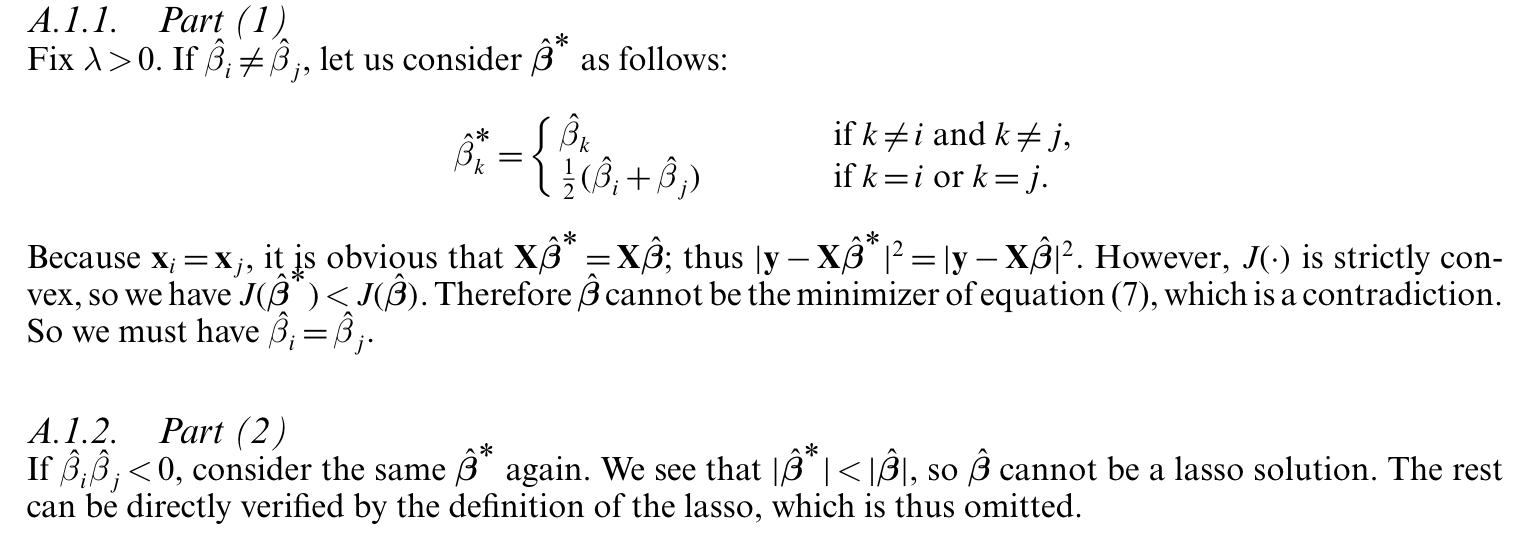
\includegraphics[width=1\textwidth]{img/image3.png}
    \end{figure}
\end{frame}

\begin{frame}{Grouping effect}
    \begin{theorem}[1]
        Given data \( (y, X) \) and parameters \( (\lambda_1, \lambda_2) \), the response \( y \) is centred and the predictors \( X \) are standardized. Let \( \hat{\beta}(\lambda_1, \lambda_2) \) be the naive elastic net estimate. Suppose that \( \hat{\beta}_i(\lambda_1, \lambda_2) \hat{\beta}_j(\lambda_1, \lambda_2) > 0 \). Define

$$
D_{\lambda_1,\lambda_2}(i, j) = \frac{1}{\lVert y \rVert_1} \left| \hat{\beta}_i(\lambda_1, \lambda_2) - \hat{\beta}_j(\lambda_1, \lambda_2) \right|;
$$

then

$$
D_{\lambda_1,\lambda_2}(i, j) \leq \frac{1}{\lambda_2} \sqrt{2(1 - \rho)},
$$

where \( \rho = x_i^T x_j \), the sample correlation.
    \end{theorem}
\end{frame}

\section{Elastic net}
    \begin{frame}{Deficiency of the naive elastic net}
    In the regression prediction setting, an accurate penalization method achieves good prediction performance through the bias–variance trade-off.\\ 
    \vspace{10pt}
    The naive elastic net estimator is a two-stage procedure: for each fixed $\lambda_2$ we first find the ridge regression coefficients, and then we do the lasso-type shrinkage along the lasso coefficient solution paths. It appears to incur a double amount of shrinkage. \\
    \vspace{10pt}
    \textbf{Double shrinkage} introduces unnecessary extra bias, compared with pure lasso or ridge shrinkage. 
    \end{frame}

    \begin{frame}{The elastic net estimate}
         Given data \( (y, X) \), penalty parameter \( (\lambda_1, \lambda_2) \) and augmented data \( (y^*, X^*) \), the naive elastic net solves a lasso-type problem
\begin{equation}
   \hat{\beta}^* = \arg\min_{\beta^*} \left\| y^* - X^* \beta^* \right\|_2^2 + \frac{\lambda_1}{\sqrt{(1 + \lambda_2)}} \left\| \beta^* \right\|_1. 
\end{equation}

The elastic net (corrected) estimates \( \hat{\beta} \) are defined by

\begin{equation}
    \hat{\beta}(\text{elastic net}) = \sqrt{(1 + \lambda_2)} \hat{\beta}^*.
\end{equation}


Recall that \( \hat{\beta}(\text{naive elastic net}) = \frac{1}{\sqrt{(1 + \lambda_2)}} \hat{\beta}^* \); thus

\begin{equation}
  \hat{\beta}(\text{elastic net}) = (1 + \lambda_2) \hat{\beta}(\text{naive elastic net}).   
\end{equation}

Hence the elastic net coefficient is a \textbf{rescaled} naive elastic net coefficient.
    \end{frame}

\begin{frame}{The elastic net estimate}
    A strong motivation for the \( (1 + \lambda_2) \)-rescaling comes from a decomposition of the ridge operator. Since the predictors \( X \) are standardized, we have

$$
\mathbf{X}^\top\mathbf{X} = \begin{pmatrix}
1 & \rho_{12} & \cdots & \rho_{1p} \\
 & 1 & \cdots & \cdot \\
 &  & \ddots & \cdot \\
 &  &  & 1
\end{pmatrix}_{p \times p},
$$

where \( \rho_{i,j} \) is sample correlation. Ridge estimates with parameter \( \lambda_2 \) are given by \( \hat{\beta}(\text{ridge}) = R\boldsymbol{y} \),

$$
R = (X^TX + \lambda_2I)^{-1}X^T.
$$



\end{frame}

\begin{frame}{The elastic net estimate}
    We can rewrite \( R \) as
\begin{equation}
   R = \frac{1}{1 + \lambda_2} R^* = \frac{1}{1 + \lambda_2} \begin{pmatrix}
\frac{1}{1+\lambda_2} & \frac{\rho_{12}}{1+\lambda_2} & \cdots & \frac{\rho_{1p}}{1+\lambda_2} \\
 & \frac{1}{1+\lambda_2} & \cdots & \cdot \\
 &  & \ddots & \cdot \\
 &  &  & \frac{1}{1+\lambda_2}
\end{pmatrix}^{-1} X^T. 
\end{equation}

\( R^* \) is like the usual OLS operator except that the correlations are shrunk by the factor \( 1/(1 + \lambda_2) \), which we call $\*decorrelation\*$. \\
\vspace{10pt}
Hence from equation (11) we can interpret the ridge operator as decorrelation followed by direct scaling shrinkage.
\end{frame}

\begin{frame}{The elastic net estimate}
    This decomposition suggests that the grouping effect of ridge regression is caused by the decorrelation step. When we combine the grouping effect of ridge regression with the lasso, the direct \( 1/(1 + \lambda_2) \) shrinkage step is not needed and is removed by rescaling.\\
    \vspace{10pt}
    Although ridge regression requires \( 1/(1 + \lambda_2) \) shrinkage to control the estimation variance effectively, in our new method, we can rely on the lasso shrinkage to control the variance and to obtain sparsity.
\end{frame}

\begin{frame}{The elastic net estimate}
    \begin{theorem}[2]
        Given data \( (y, X) \) and parameters \( (\lambda_1, \lambda_2) \), then the elastic net estimates \( \hat{\beta} \) are given by
\begin{equation}
   \hat{\beta} = \arg\min_{\beta} \left[ \beta^T \left( \frac{X^TX + \lambda_2 I}{1 + \lambda_2} \right) \beta - 2y^T X\beta \right] + \lambda_1 \lVert \beta \rVert_1. 
\end{equation}

It is easy to see that

\begin{equation}
   \hat{\beta}(\text{lasso}) = \arg\min_{\beta} \left[ \beta^T (X^TX) \beta - 2y^T X\beta \right] + \lambda_1 \lVert \beta \rVert_1. 
\end{equation}
    \end{theorem}
\end{frame}

\begin{frame}{The elastic net estimate}
\textbf{proof:}
    Let \( \hat{\beta} \) be the elastic net estimates. By definition and equation (10) we have

$$
\hat{\beta} = \arg\min_{\beta} \left[ \frac{1}{\sqrt{(1 + \lambda_2)}} \left\| y^* - X^* \beta \right\|_2^2 + \frac{\lambda_1}{\sqrt{(1 + \lambda_2)}} \left\| \beta \right\|_1 \right]
$$

$$
= \arg\min_{\beta} \beta^T \left( \frac{X^TX + \lambda_2 I}{1 + \lambda_2} \right) \beta - 2 y^T X\beta + \frac{\lambda_1}{1 + \lambda_2} \left\| \beta \right\|_1. \qquad (14)
$$

Substituting the identities

$$
X^{*T} X^* = \left( \frac{X^TX + \lambda_2 I}{1 + \lambda_2} \right),
$$


\end{frame}

\begin{frame}{The elastic net estimate}
   \textbf{(continued)} $$
y^{*T} X^* = \frac{y^TX}{\sqrt{(1 + \lambda_2)}},
$$

$$
y^{*T} y^* = y^T y
$$

into equation (14), we have

$$
\hat{\beta} = \arg\min_{\beta} \frac{1}{1 + \lambda_2} \left[ \beta^T \left( \frac{X^TX + \lambda_2 I}{1 + \lambda_2} \right) \beta - 2 y^TX\beta + \lambda_1 \left\| \beta \right\|_1 \right] + y^T y
$$

$$
= \arg\min_{\beta} \beta^T \left( \frac{X^TX + \lambda_2 I}{1 + \lambda_2} \right) \beta - 2 y^TX\beta + \lambda_1 \left\| \beta \right\|_1.
$$
\end{frame}

\begin{frame}{Connections with univariate soft thresholding}
The lasso is a special case of the elastic net with \( \lambda_2 = 0 \). The other interesting special case of the elastic net emerges when \( \lambda_2 \to \infty \). By theorem 2, \( \hat{\beta} \to \hat{\beta}(\infty) \) as \( \lambda_2 \to \infty \), where

$$
\hat{\beta}(\infty) = \arg\min_{\beta} \left[ \beta^T \beta - 2y^T X\beta + \lambda_1 \lVert \beta \rVert_1 \right].
$$
\end{frame}

\begin{frame}{Connections with univariate soft thresholding}
   \( \hat{\beta}(\infty) \) has a simple closed form

$$
\hat{\beta}(\infty)_i = \left( \lvert y^T X_i \rvert - \frac{\lambda_1}{2} \right)_+ \text{sgn}(y^T X_i), \quad i=1,2,...,p. \quad (15)
$$

Observe that \( y^T X_i \) is the univariate regression coefficient of the ith predictor and \( \hat{\beta}(\infty) \) are the estimates by applying soft thresholding on univariate regression coefficients; thus equation (15) is called univariate soft thresholding (UST). 
\end{frame}

\begin{frame}{Computation: the algorithm LARS-EN}
    In a word, we do not explicitly use $X^*$ to compute all the quantities in algorithm LARS. It is also economical to record only the non-zero coefficients and the active variables set at each LARS-EN step.
\end{frame}

\begin{frame}{Choice of tuning parameters}
    For each fixed $\lambda_2$, the elastic net is solved by our algorithm LARS-EN; hence similarly we can use the number of the LARS-EN steps (k) as the second tuning parameter besides $\lambda_2$.
\end{frame}
